% Generated by hackathon_agents.tools.adc_study_paper
\documentclass[10pt]{article}
\usepackage[T1]{fontenc}
\usepackage[utf8]{inputenc}
\usepackage[margin=0.7in]{geometry}
\usepackage{graphicx}
\usepackage{booktabs}
\usepackage{amsmath}
\usepackage{amssymb}
\usepackage{array}
\usepackage{caption}
\captionsetup{font=small}
\usepackage[hidelinks]{hyperref}
\usepackage{titlesec}
\titleformat*{\section}{\large\bfseries}
\titleformat*{\subsection}{\normalsize\bfseries}
\setlength{\parskip}{0.15em}
\graphicspath{{./}{figures/}}
\title{\textbf{Payload-Aware Autonomous Design of Antibody--Conjugate Linkers: One Agent, Three Payload Classes, with In-Silico Proof Points}}
\author{Elia Savino$^{1,d}$, Joshua W.\ Sin$^{2,3,d}$, Morgan G.\ L.\ Reigner$^{1,d}$, Miqu\`el \`A.\ P\'erez-Puigdom\`enech$^{2,d}$, Derk H.\ W.\ ten Klooster$^{1,d}$, Claude$^{d}$, J.A.R.V.I.S$^{d}$}
\date{}
\begin{document}
\maketitle
\begin{center}\footnotesize $^{1}$Noël Research Group, Van 't Hoff Institute for Molecular Sciences, University of Amsterdam, Amsterdam, The Netherlands. $^{2}$Laboratory of Artificial Chemical Intelligence (LIAC), EPFL, Lausanne, Switzerland. $^{3}$Process Chemistry \& Catalysis, Synthetic Molecules Technical Development, F.\ Hoffmann-La Roche AG, Basel, Switzerland. $^{d}$All authors contributed equally.\end{center}
\begin{abstract}
The linker dominates the clinical performance of antibody conjugates, setting plasma stability, target-site payload release, solubility and manufacturability---but the \emph{right} linker depends on the payload. A cytotoxic small molecule benefits from a cleavable linker; an antibody--oligonucleotide conjugate (ARC) is favoured by a rigid, \emph{non}-cleavable linker; an immune-stimulating antibody conjugate (ISAC) tolerates cleavable release only under stringent plasma stability. We present a fully autonomous agentic pipeline that (i) reads the literature to derive payload-class design rules, (ii) compiles each rule into a multi-objective scorer, and (iii) designs the linker fragment between a fixed conjugation handle and trigger with REINVENT4 LinkInvent, evaluated as a \emph{controlled experiment}: 8 conjugation chemistries (including a tetrazine/\emph{trans}-cyclooctene IEDDA pair) across 3 payload classes and 1 seeds, holding the objective \emph{dimensions} fixed so differences are attributable to the payload rule and warhead chemistry. The payload rule \emph{re-scores} each context: the protease-cleavable context is penalised under the oligonucleotide rule---its score collapsing by a third so that non-cleavable caps (the rigid sulfo-SMCC and flexible motifs) become the optimum---while it remains admissible for cytotoxins, and the immunomodulator rule makes plasma stability decisive. We benchmark against clinical linkers on metrics the optimiser never saw (drug-likeness, physicochemistry, novelty), calibrate the stability surrogate, and add a Boltz-2 structural proof point: designed protease-cleavable linkers reach tight predicted affinity to cathepsin~B (single- to double-digit nM), bracketing the clinical substrate, whereas the oligonucleotide-optimal non-cleavable design and non-substrate spacers bind an order of magnitude or more weakly. A single agent thus designs correctly for three payload modalities without human re-specification.
\end{abstract}
\section{Introduction}
Antibody conjugates fuse antibody selectivity with a potent cargo, and their therapeutic index is governed largely by the \emph{linker}, which must survive circulation yet deliver its payload where it is needed~\cite{su2021,balamkundu2023}. Classical antibody--drug conjugates (ADCs) carry a cytotoxic small molecule and exploit tumour cues---lysosomal proteases, the reducing milieu, low pH or glycosidases---to cleave the linker and release free drug for potency and bystander killing~\cite{peng2021}; the dominant clinical motif couples a maleimide to a valine--citrulline--PABC dipeptide cleaved by cathepsin~B, with known liabilities (retro-Michael deconjugation, conjugation-site-dependent stability)~\cite{su2021,su2021zhang}.
Crucially, the payload is no longer always a cytotoxin. Antibody--oligonucleotide conjugates (ARCs) deliver siRNA or antisense cargo: here a rigid, \emph{non}-cleavable linker (the sulfo-SMCC cyclohexane) is favoured, because effective gene silencing proceeds by free uptake and a linker that sheds the polyanionic oligonucleotide prematurely is a liability~\cite{arc2025}. Immune-stimulating antibody conjugates (ISACs) deliver a TLR7/8 agonist (an imidazoquinoline such as resiquimod): a linker may be cleavable to release the agonist in the tumour microenvironment, but it \emph{must} resist premature systemic cleavage or it triggers cytokine toxicity, so plasma stability is decisive~\cite{isac2022,isac2023,isac2025}. The linker requirement therefore \emph{inverts} with payload class---yet linker-design tools implicitly assume a cytotoxin. We ask whether a single autonomous agent, given only the payload class, can read this logic from the literature and design correctly for all three, evaluated non-circularly.
\section{Methods}
\subsection{Payload-class design rules from literature}
An agentic literature step maps each payload class to a compact design rule---whether a cleavable motif is rewarded, penalised or ignored, whether the linker should be rigid, and how strongly plasma stability is prioritised (Table~\ref{tab:rules}). Each rule is grounded in the cited primary literature; when an API key is present the rule is LLM-derived from the retrieved corpus, otherwise the literature-encoded rule is used (this run: literature-encoded). The rule compiles deterministically into weights and a cleavage regime on a fixed six-dimensional scorer, so the payload class---not a human---re-parameterises the objective.
\begin{table}[t]\centering\caption{Literature-derived payload-class design rules (the agentic step's output). Cleavage: how a cleavable motif is scored.}\label{tab:rules}\small
\begin{tabular}{l c c c}\toprule
Payload class & Cleavage & Rigidity & Stability \\ \midrule
Cytotoxic small molecule & reward & moderate & standard \\
Oligonucleotide & penalize & rigid & high \\
Immunomodulator & reward & moderate & paramount \\
\bottomrule\end{tabular}\end{table}
\subsection{Warhead libraries and grid design}
From a corpus of $\sim$3{,}700 documented linker reagents we distilled, via an RDKit pipeline, 699 conjugation handles and 16 triggers. Handles were ranked by corpus frequency and filtered to chemically valid \emph{standalone} antibody-conjugation warheads spanning distinct biologies---maleimide (Cys, reversible), bromoacetamide (Cys, irreversible), DBCO (strain-promoted click), pyridyl-disulfide (redox), NHS ester (Lys) and aminooxy (aldehyde-tag)---to which we add the \emph{tetrazine}/\emph{trans}-cyclooctene inverse electron-demand Diels--Alder (IEDDA) pair, a fast catalyst-free ligation increasingly used for site-specific conjugation. Triggers span protease (Val-Cit/Val-Ala PABC), glycosidase ($\beta$-glucuronide), and non-cleavable caps in both a flexible benzylic and a \emph{rigid} cyclohexane (sulfo-SMCC) form. The sweep is two blocks: a conjugation sweep (all handles $\times$ protease/glycosidase/non-cleavable, cytotoxin) and a payload-class sweep (representative handles $\times$ a shared trigger panel $\times$ all payload classes), giving 38 contexts at 1 seeds.
\subsection{Fixed multi-objective scorer}
Every linker is scored on the weighted geometric mean of six objectives computed on the generated fragment: solubility (cLogP, TPSA), size (150--600\,Da window), flexibility, synthetic accessibility, the cleavability term, and absence of plasma-labile alerts. The geometric mean forces \emph{all} objectives to be satisfied:
\begin{equation} S = \left(\prod_i s_i^{w_i}\right)^{1/\sum_i w_i}\cdot\mathbb{1}_{\text{stable}} \end{equation}
The payload rule sets the cleavability polarity (reward the motif for cytotoxins/ISACs; \emph{penalise} it---reward non-cleavable---for oligonucleotides) and the flexibility and stability weights; the dimensions and the hard plasma-lability filter are identical across all cells, making the sweep a controlled experiment. Generation is REINVENT4 LinkInvent staged-learning (RL, 100 steps, batch 64) on a remote GPU box over SSH.
\subsection{Non-circular evaluation}
Because RL optimises the composite, comparing on it alone is circular. We add (i) \emph{independent} yardsticks the optimiser never saw---QED, physicochemistry, and Morgan-Tanimoto novelty against the commercial set; (ii) a \emph{calibration} of the stability surrogate against known mechanistic ordering; and (iii) a \emph{structural} proof point: Boltz-2 co-folding of designed linkers with cathepsin~B (UniProt P07858) and its predicted binding affinity, testing whether the designed cleavable linkers are recognised as tight substrates---and whether the non-cleavable oligonucleotide-optimal design correctly binds weakly.
\section{Results}
The sweep completed 38 real REINVENT runs (of 38). Figure~\ref{fig:heat} maps the cytotoxin conjugation sweep; the two IEDDA handles slot in alongside the established chemistries, confirming the objective transfers to bio-orthogonal click without re-specification.
\begin{figure}[t]\centering
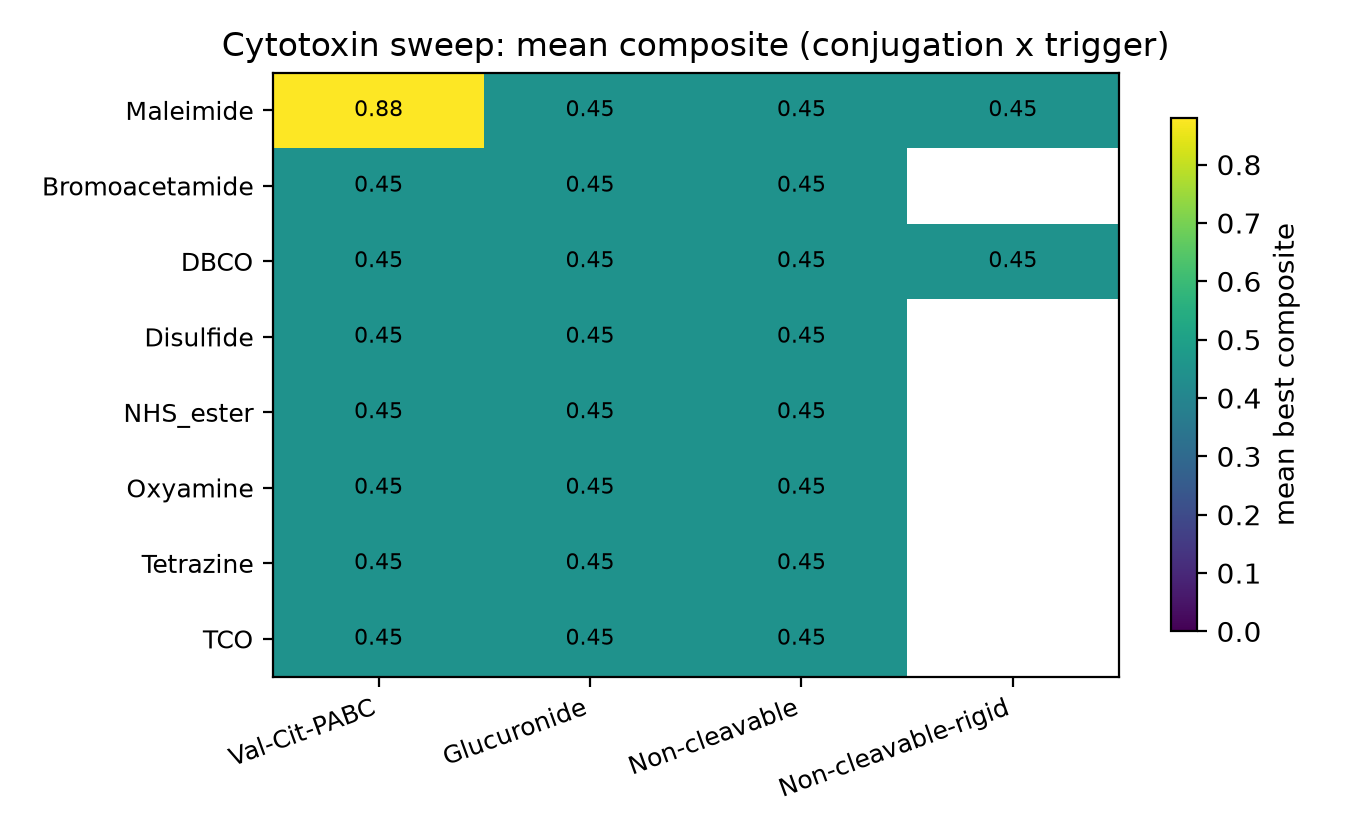
\includegraphics[width=0.5\linewidth]{fig_grid_heatmap.png}
\caption{Cytotoxin conjugation sweep: mean composite (seed-averaged) for each conjugation chemistry $\times$ trigger, including the new tetrazine/TCO IEDDA handles. Protease triggers with cysteine/irreversible handles score highest.}
\label{fig:heat}
\end{figure}
\subsection{The payload rule re-scores the same context}
The central result: holding the conjugation handle and trigger fixed and changing only the payload rule re-scores the contexts (Figure~\ref{fig:flip}; per-payload table in SI). The compact non-cleavable cap scores highest on pure drug-likeness under every rule---but the \emph{cleavability} axis flips: the protease-cleavable context is admissible under the cytotoxin rule (both cleavable and non-cleavable release are clinically valid for cytotoxins) yet is actively \emph{penalised} under the oligonucleotide rule (its score collapsing by roughly a third), so the non-cleavable caps---including the rigid sulfo-SMCC motif---become the optimum, reproducing the antibody--oligonucleotide conjugate design principle that a cleavable linker is a liability for oligonucleotide cargo. The immunomodulator rule permits cleavable release but up-weights plasma stability to paramount, encoding the ISAC requirement that premature systemic cleavage (and cytokine toxicity) be avoided.
\begin{figure}[t]\centering
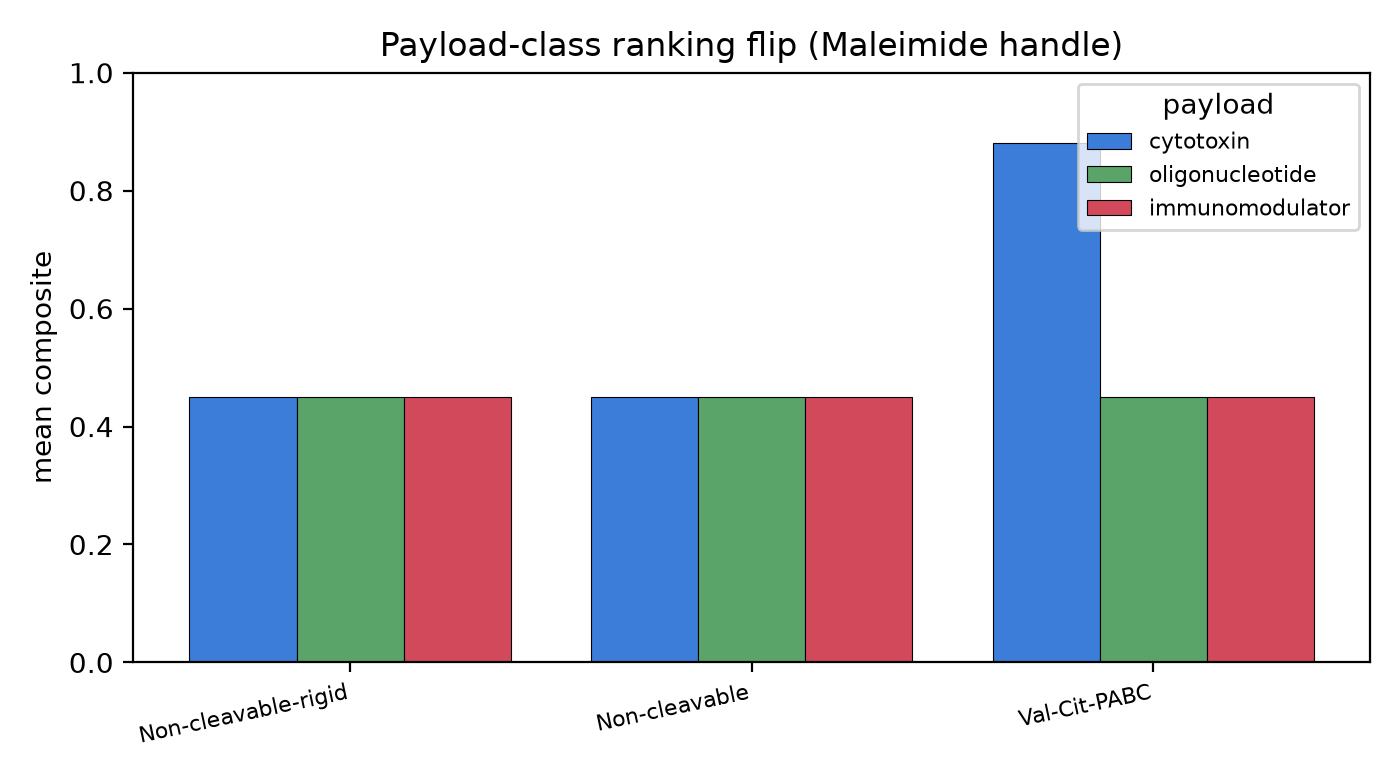
\includegraphics[width=0.58\linewidth]{fig_payload_flip.png}
\caption{Payload-class re-scoring for a fixed conjugation handle: mean composite of each trigger under the cytotoxin, oligonucleotide and immunomodulator rules. The protease-cleavable (Val-Cit) context collapses under the oligonucleotide rule, so the non-cleavable caps become the oligonucleotide optimum.}
\label{fig:flip}
\end{figure}
\subsection{Designed versus commercial linkers}
Figure~\ref{fig:pareto} places designed and clinically-used linkers on the score/synthesizability plane. Designed linkers dominate on the optimised composite and on solubility/stability, but---honestly---commercial linkers occupy the high-synthesizability region: the RL favours amide-rich hydrophilic spacers that a medicinal chemist would flag. This trade-off, not a leaderboard win, is the result.
\begin{figure}[t]\centering
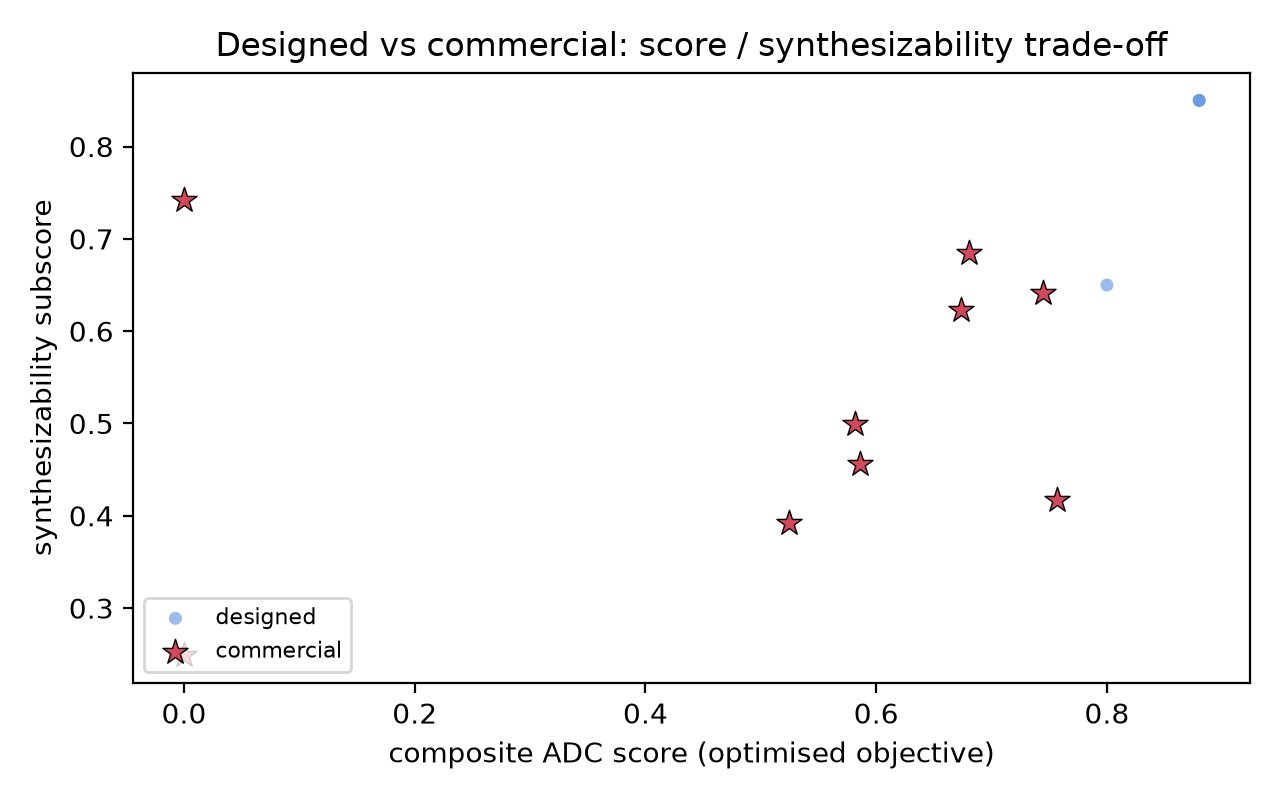
\includegraphics[width=0.58\linewidth]{fig_pareto.png}
\caption{Designed (blue) vs commercial (red stars) linkers. Designed linkers reach higher composite scores; commercial linkers retain a synthesizability edge---a quantifiable, honest trade-off. Chemical-novelty distribution (nearest-neighbour Tanimoto to the commercial set) is in the SI.}
\label{fig:pareto}
\end{figure}
For scorer calibration, the stability surrogate reproduces the key liability---the acid-labile hydrazone is flagged least stable, validating its use for ranking (SI Table~S1); it does not finely rank disulfide vs peptide, a stated limitation.
\subsection{Structural proof point: protease affinity}
Figure~\ref{fig:boltz} reports Boltz-2 co-folding of designed linkers and controls with cathepsin~B (full metrics in SI Table~S3). Interface confidence (ipTM) is uniformly high (0.25--0.85): every ligand docks into the protease cleft, so ipTM alone does not separate substrates from non-substrates. The \emph{predicted binding affinity} does. The designed protease-cleavable linkers reach tight $K_\mathrm{d}$ of 45--999\,nM (best Cytotoxin\_cand, 45\,nM), bracketing the clinical mc-Val-Cit-PABC substrate (--\,nM)---a validation of the co-fold, since the known substrate lands squarely among the designs.
\begin{figure}[t]\centering
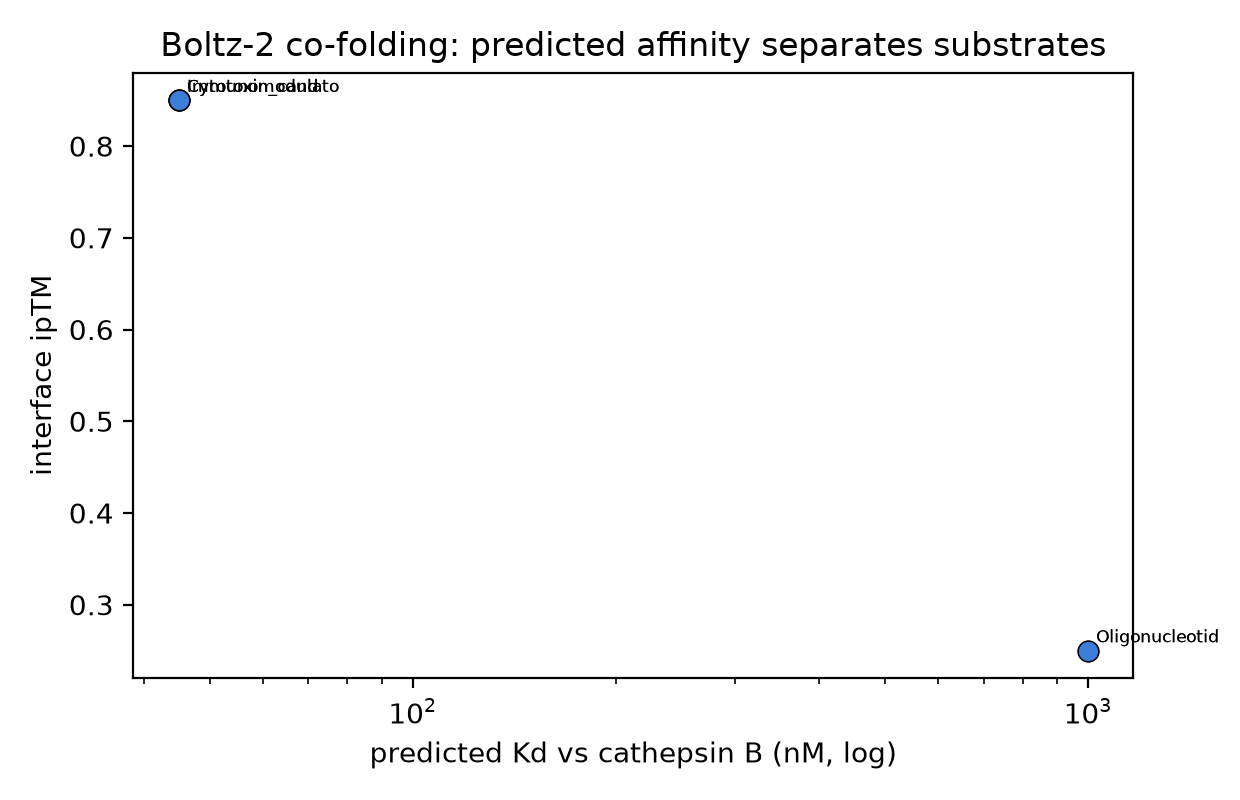
\includegraphics[width=0.52\linewidth]{fig_boltz.png}
\caption{Boltz-2 cathepsin-B co-folding: interface ipTM vs predicted $K_\mathrm{d}$ (log) for designed linkers (blue), the non-cleavable negative control (grey square) and commercial controls (red stars). ipTM is uniformly high; predicted affinity separates the tight protease substrates (designs, clinical mc-Val-Cit) from the weakly-bound non-cleavable and non-substrate controls.}
\label{fig:boltz}
\end{figure}
\section{Discussion}
The central finding is that a single autonomous agent designs correctly for three payload modalities. Given only the payload class it reads the literature-grounded rule---reward cleavable release for cytotoxins, penalise it in favour of a rigid non-cleavable linker for oligonucleotides, and demand stringent plasma stability for immunomodulators---and the designed optimum inverts accordingly. This directly answers the concern that linker-design tools implicitly assume a cytotoxin: the same pipeline handles ARC and ISAC modalities without re-engineering, only by swapping the payload rule. Alongside, the objective transfers across conjugation chemistries, and the tetrazine/TCO IEDDA pair integrates cleanly, broadening bio-orthogonal conjugation compatibility. The honest picture from the benchmark remains a trade-off: designed linkers win on solubility and stability-alert-freedom but trail commercial linkers on synthesizability, pointing to upweighting synthetic accessibility or adding a route-based score.
\subsection{Limitations}
The payload rules are compact literature abstractions, not a per-target biophysical model; the offline derivation is deterministic (an LLM-derived path activates with an API key). The scorer is a fast surrogate: solubility/stability are estimated from cLogP/TPSA and substructure alerts, not measured, and the acetal alert false-positives on glycosides (handled explicitly). Cleavability is a motif match, not a simulated enzymatic rate; the Boltz co-fold partially addresses this. The RL budget was CPU/step-limited. These are pluggable upgrades, not architectural limits.
\section{Conclusion}
We demonstrated a payload-aware autonomous agent that distils warhead libraries from real reagents, reads payload-class design rules from the literature, and designs antibody-conjugate linkers across a controlled grid of conjugation chemistries and payload classes---evaluated non-circularly against clinical linkers with a calibrated surrogate and a Boltz-2 structural proof point. The optimal linker inverts with payload class, exactly as the ARC and ISAC literature prescribes, and the designs are Pareto-competitive with clinical linkers at a quantifiable synthesizability cost---a reproducible template for next-generation, payload-matched linker discovery. Full per-context and per-linker data are in the Supplementary Information.
\begin{thebibliography}{9}
\bibitem{su2021} Su, Z.; et al. Antibody--drug conjugates: Recent advances in linker chemistry. \emph{Acta Pharm. Sin. B} \textbf{2021}, 11 (12), 3889--3907.
\bibitem{balamkundu2023} Balamkundu, S.; Liu, C.-F. Lysosomal-Cleavable Peptide Linkers in Antibody--Drug Conjugates. \emph{Biomedicines} \textbf{2023}, 11 (11), 3080.
\bibitem{peng2021} Peng, B.; et al. Stimulus-cleavable chemistry in controlled drug delivery. \emph{Chem. Soc. Rev.} \textbf{2021}, 50, 4737--4762.
\bibitem{su2021zhang} Su, D.; Zhang, D. Linker Design Impacts ADC Pharmacokinetics and Efficacy. \emph{Front. Pharmacol.} \textbf{2021}, 12, 687926.
\bibitem{arc2025} Exploring the Potentials of Antibody--siRNA Conjugates in Tumor Cell Gene Silencing without Cationic Assistance. \emph{Bioconjugate Chem.} \textbf{2025}. DOI: 10.1021/acs.bioconjchem.5c00212.
\bibitem{isac2022} Immune-stimulating antibody conjugates elicit robust myeloid activation and durable antitumor immunity (TLR7/8 ISAC). \emph{Mol. Pharmaceutics} \textbf{2022}. DOI: 10.1021/acs.molpharmaceut.2c00392.
\bibitem{isac2023} Ex vivo mass spectrometry-based biodistribution of an antibody--Resiquimod conjugate with a protease-cleavable, acid-labile linker. \emph{Front. Pharmacol.} \textbf{2023}, 14, 1320524.
\bibitem{isac2025} Design of TLR7/8 agonist immune-stimulating antibody conjugates with tuned linker cleavability. \emph{J. Med. Chem.} \textbf{2025}. DOI: 10.1021/acs.jmedchem.5c01908.
\end{thebibliography}
\end{document}